% Copyright 2004 by Till Tantau <tantau@users.sourceforge.net>.
%
% In principle, this file can be redistributed and/or modified under
% the terms of the GNU Public License, version 2.
%
% However, this file is supposed to be a template to be modified
% for your own needs. For this reason, if you use this file as a
% template and not specifically distribute it as part of a another
% package/program, I grant the extra permission to freely copy and
% modify this file as you see fit and even to delete this copyright
% notice. 

\documentclass[11pt]{beamer}
\setbeamertemplate{caption}[numbered]
% Replace the \documentclass declaration above
% with the following two lines to typeset your 
% lecture notes as a handout:
%\documentclass{article}
%\usepackage{beamerarticle}
\usepackage[utf8]{inputenc}
\usepackage[noend]{algpseudocode}
\usepackage[T1]{fontenc}
\usepackage{algorithmicx}
\usepackage{amsmath}
\usepackage{mathtools}
\usepackage[french,british]{babel}
\usepackage{algorithm}

\usepackage[font=scriptsize,skip=5pt]{caption}
%\setlength{\textfloatsep}{1.0pt plus 1.0pt minus 2.0pt}

\setbeamertemplate{footline}[frame number]

% There are many different themes available for Beamer. A comprehensive
% list with examples is given here:
% http://deic.uab.es/~iblanes/beamer_gallery/index_by_theme.html
% You can uncomment the themes below if you would like to use a different
% one:
%\usetheme{AnnArbor}
%\usetheme{Antibes}
%\usetheme{Bergen}
%\usetheme{Berkeley}
%\usetheme{Berlin}
%\usetheme{Boadilla}
%\usetheme{boxes}
%\usetheme{CambridgeUS}
%\usetheme{Copenhagen}
%\usetheme{Darmstadt}
%\usetheme{default}
%\usetheme{Frankfurt}
%\usetheme{Goettingen}
%\usetheme{Hannover}
%\usetheme{Ilmenau}
%\usetheme{JuanLesPins}
%\usetheme{Luebeck}
%\usetheme{Madrid}
%\usetheme{Malmoe}
%\usetheme{Marburg}
\usetheme{Montpellier}
%\usetheme{PaloAlto}
%\usetheme{Pittsburgh}
%\usetheme{Rochester}
%\usetheme{Singapore}
%\usetheme{Szeged}
%\usetheme{Warsaw}

%=====================================================Slide 1
\titlegraphic{
\begin{figure}[!htb]
\minipage{0.07\textwidth}
  
\includegraphics[width=\linewidth]{images/ctu-logo}
\endminipage\hfill
\minipage{0.07\textwidth}
  
\includegraphics[width=\linewidth]{images/ifi-logo}
\endminipage\hfill
\minipage{0.07\textwidth}
  
\includegraphics[width=\linewidth]{images/auf-logo}
\endminipage\hfill
\minipage{0.07\textwidth}
  
\includegraphics[width=\linewidth]{images/unh-logo}
\endminipage\hfill
\end{figure}
}

\title{Algorithme parallèle de Descente de gradient stochastique multi-classes pour la classification d'images
}

\author[1]{Réalisateur : NGUYEN Quoc Khai, promotion 17, IFI \\[\baselineskip]
Superviseurs : DO Thanh Nghi(CTU), PHAM Nguyen Khang(CTU) et HO Tuong Vinh(IFI)
}

\date{Stage M2 réalisé à la laboratoire IDPL, CTU, Cantho, 2014}


% - Either use conference name or its abbreviation.
% - Not really informative to the audience, more for people (including
%   yourself) who are reading the slides online

\subject{sgd pour la classification d'images}
% This is only inserted into the PDF information catalog. Can be left
% out. 

% If you have a file called "university-logo-filename.xxx", where xxx
% is a graphic format that can be processed by latex or pdflatex,
% resp., then you can add a logo as follows:

% \pgfdeclareimage[height=0.5cm]{university-logo}{university-logo-filename}
% \logo{\pgfuseimage{university-logo}}

% Delete this, if you do not want the table of contents to pop up at
% the beginning of each subsection:
\AtBeginSection[]
{
  \begin{frame}<beamer>{Plan de présentation}
    \tableofcontents[currentsection, currentsubsection]
  \end{frame}
}

% Let's get started
\begin{document}
\begin{otherlanguage}{french}
\begin{frame}
  \titlepage
\end{frame}


%=====================================================Slide 2
\begin{frame}{Plan de présentation}
  \tableofcontents
  % You might wish to add the option [pausesections]
\end{frame}


\section{Introduction générale}
%=====================================================Slide 4
\begin{frame}{Introduction générale}
\begin{itemize}
\item La classification d'images est importante : la reconnaissance des scènes, la reconnaissance des chiffres sur des chèques, la reconnaissance des codes postaux pour la classification automatique des courriers, la reconnaissance des visages pour l'authentification, etc.

\item Pas encore une méthode optimale

\item SVM (Support vector machine) est la plus populaire dans le domaine de classification, régression.

\end{itemize}
\end{frame}

%=====================================================Slide 6
\begin{frame}{Introduction - classification d'images}
\begin{figure}[ht!]
\centering
\includegraphics[width=105mm]{images/classification}
\caption{La classification d'image}
\vspace{-2.0em}
\label{fig:classification}
\end{figure}
\end{frame}

%=====================================================Slide 5
\begin{frame}{Introduction - méthode SVM}

\begin{figure}[ht!]
\centering
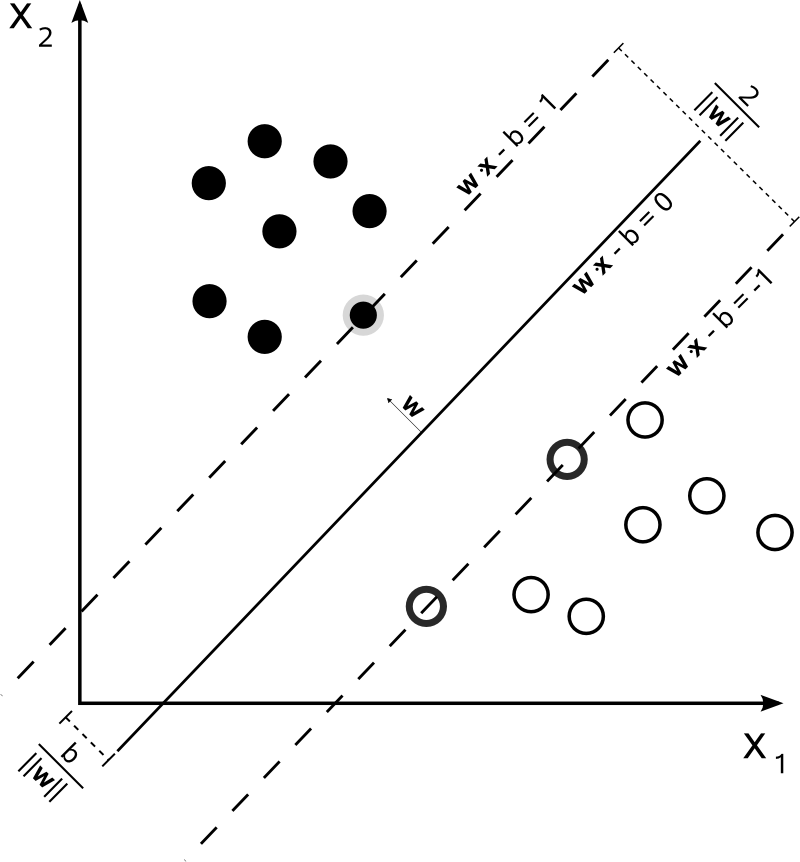
\includegraphics[width=25mm]{images/svm}
\caption{Méthode SVM pour la classification}
\vspace{-2.0em}
\label{fig:svm}
\end{figure}

\begin{itemize}
\item Une méthode de classification du domaine d'apprentissage automatique
\item Classer des données en classes différentes. L'image \ref{fig:svm} est la classification binaire 
\item Comment l'appliquer pour la classification d'images ?
\end{itemize}
\end{frame}

%=====================================================Slide 6
\begin{frame}{Introduction - processus de SVM pour classification d'images}
\begin{enumerate}
\item Extraction des caractéristiques des images : obtenir des vecteurs de caractéristiques (SIFT)
\item Construire un dictionnaire, calculer le fréquence de chaque mot apparait dans chaque image (histogramme) pour préparer des entrées pour la méthode SVM : obtenir des histogrammes de chaque image (BOW)
\item Application SVM pour l'apprentissage automatique sur des histogrammes pour la classification
\end{enumerate}
\end{frame}


%=====================================================Slide 6
\begin{frame}{Introduction - processus de SVM pour classification d'images}
\begin{figure}[ht!]
\centering
\includegraphics[width=105mm]{images/svm-processus}
\caption{Processus de SVM pour la classification d'image}
\vspace{-2.0em}
\label{overflow}
\end{figure}
\end{frame}

%=====================================================Slide 6
\begin{frame}{Introduction - méthode SGD}
\begin{itemize}
\item SVM est satisfait pour la classification d'image, mais cette méthode est lent. SGD est une version simple de SVM

$\rightarrow$ SGD est une bonne choix pour améliorer la vitesse
\item Même processus avec SVM pour la classification d'image. SGD remplace SVM dans l'étape 3, l'étape apprentissage automatique.
\item Nous développons et parallélisons un algorithme de classification SGD multi-classes et cette méthode est bien adapté à la classification d'image de grand taille
\end{itemize}
\end{frame}


\section{État de l'art}
\subsection{Extraction des caractéristiques}
%=====================================================Slide 8
\begin{frame}{Introduction pour extraction des caractéristiques}
\begin{itemize}
\item Point d'intérêt : les points fixés quand l'image est changé de scale, la taille, la rotation.
\item Extraction des caractéristiques (visual features extraction) : après la détection de points d'intérêt, calculer le vecteur caractéristique sur chaque zone autour des points détectés.
\item Le vecteur caractéristique contient : l'orientation de l'arête ou la magnitude du gradient au point d'intérêt.
\item Les méthodes comme SIFT comprend l'étape détection des points d'intérêt et aussi l'extraction de caractéristiques
\end{itemize}
\end{frame}

\subsubsection*{SIFT}
%=====================================================Slide 9
\begin{frame}{Méthode SIFT}
Méthode SIFT peut être résumé en 4 étapes principales :
\begin{enumerate}
\item Détection des points d'intérêts
\item Localisation précise de points d'intérêt
\item Assignation d'orientation
\item Descripteur de point d'intérêt
\end{enumerate}

\begin{figure}[!htb]
\centering
\minipage{0.30\textwidth}
\includegraphics[width=\linewidth]{images/kv}
\caption{Image originale}
\endminipage\hfill
\minipage{0.30\textwidth}
\includegraphics[width=\linewidth]{images/kv-key}
\caption{Détection de points d'intérêt}
\endminipage\hfill
\end{figure}

\end{frame}

%=====================================================Slide 10
\begin{frame}{Méthode SIFT - Extraction des caractéristiques}

\begin{figure}[ht!]
\centering
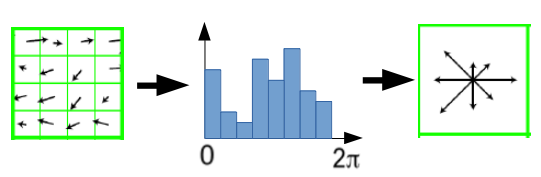
\includegraphics[width=65mm]{images/sift_hist}
\caption{Assignation d'orientation}
\label{max_margin}
\end{figure}

\begin{figure}[ht!]
\centering
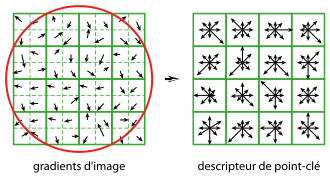
\includegraphics[width=55mm]{images/siftdescriptor}
\caption{Descripteur de caractéristiques}
\label{max_margin}
\end{figure}

\end{frame}

%=====================================================Slide 11
\subsubsection*{Sac de mots visuels}
\begin{frame}{Methode Sac de mots visuels}
Cette méthode peut diviser en 5 étapes :
\begin{enumerate}
\item Détection des points d'intérêts
\item Extraction des caractéristiques
\item Clustering des caractéristiques
\item Construire un dictionnaire a partir des clusters
\item Représenter des images par des histogrammes
\end{enumerate}
\end{frame}

%=====================================================Slide 12
\begin{frame}{Methode Sac de mots visuels - résume}

\begin{figure}[ht!]
\centering
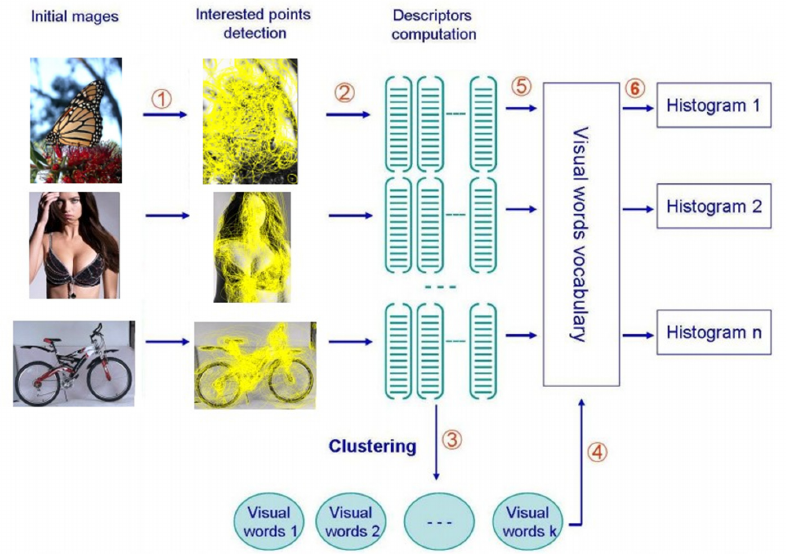
\includegraphics[width=85mm]{images/bow}
\caption{Descripteur de caractéristiques}
\label{max_margin}
\end{figure}

\end{frame}

\subsection{Apprentissage automatique}
%=====================================================Slide 13
\begin{frame}{Introduction pour apprentissage automatique}
\begin{itemize}
\item Permet aux machines d'apprendre à partir des données
\item Remplir des tâches qu'il est difficile ou impossible de remplir par des moyens algorithmiques plus classiques
\item Généraliser des données limite afin de données des réactions intelligentes sur des nouveaux exemples
\item SVM est populaire dans le domaine de classification.
\end{itemize}
\end{frame}

\subsubsection*{SVM}
%=====================================================Slide 14
\begin{frame}{Méthode SVM}
\begin{itemize}
\item Méthode d'apprentissage supervisé important
\item $m$ exemples d'entrées $x_1, x_2, ..., x_m$, de $N$ dimensions
\item Label $y_i$ : $y_1, y_2, ..., y_m$ $(y_i \in \{-1,1\})$
\item Cherche l'hyperplan optimal, séparer les points (les données) en deux parties
\end{itemize}

\begin{figure}[ht!]
\centering
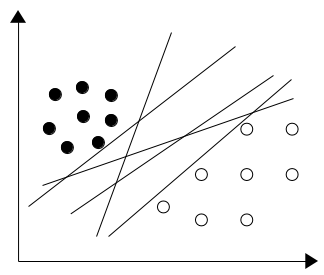
\includegraphics[width=35mm]{images/separating_lines}
\caption{Classification linéaire}
\label{slines}
\end{figure}

\end{frame}

%=====================================================Slide 15
\begin{frame}{Méthode SVM - séparateur}
\begin{itemize}
\item L'hyperplan $w=[w_1,w_2,...,w_n]$ et $b$ : $x^T.w - b = 0$
\item L'hyperplan optimal : maximiser le margin
\item 2 supports hyperplans $x^T.w - b = 1$ et $x^T.w - b = -1$
\end{itemize}

\begin{figure}[ht!]
\centering
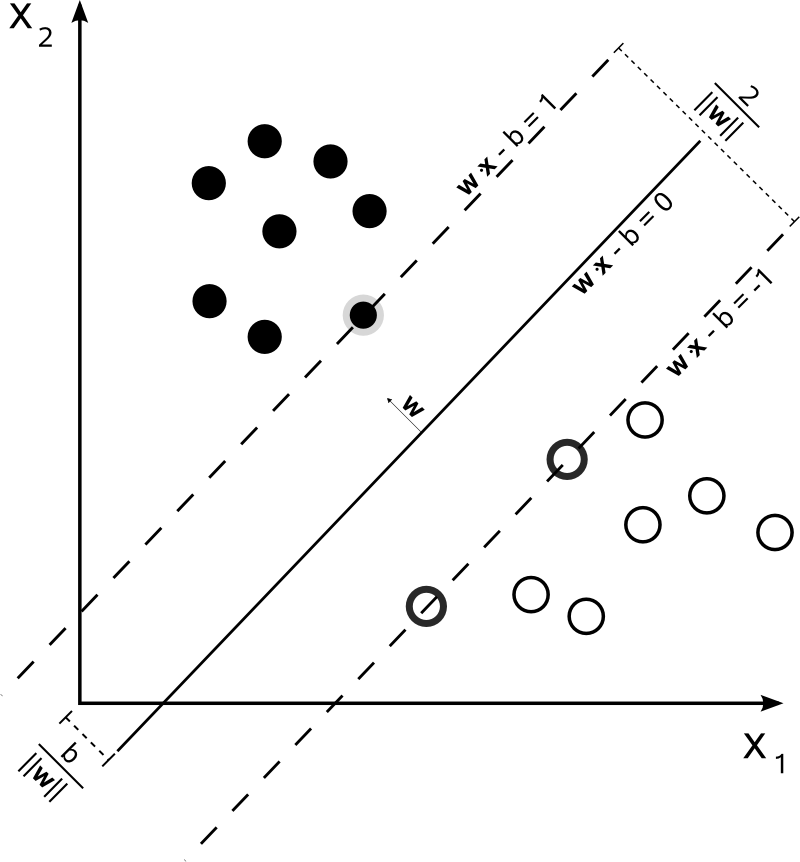
\includegraphics[width=35mm]{images/margin}
\caption{L'hyperplan optimal}
\label{max_margin}
\end{figure}

\end{frame}

%=====================================================Slide 16
\begin{frame}{Méthode SVM - classification}
Par rapport à 2 supports hyperplans parallèles (voir l'image \ref{max_margin}), la classification est réalisée grâce aux \ref{f1} et \ref{f2}.
\begin{equation}
x_i.w - b \geq +1, \Rightarrow y_i = 1
\label{f1}
\end{equation}

\begin{equation}
x_i.w - b \leq -1, \Rightarrow y_i = -1
\label{f2}
\end{equation}

Comment trouver $w$ et $b$ ?

\end{frame}

%=====================================================Slide 17
\begin{frame}{Méthode SVM - programme de quadratique}

Chercher la solution du programme de quadratique \ref{f5} pour obtenir $w$ et $b$

\begin{equation}
\begin{split}
\mbox{min}\quad \Psi(w, b, z) = \frac{1}{2} ||w||^2 + c.\sum\limits_{i=1}^m z_i\quad \\ \mbox{s.t} \quad y_i.(x_i.w - b) + z_i \geq 1 \\ \mbox{et} \quad z_i \geq 0
\end{split}
\label{f5}
\end{equation}

\end{frame}







\subsubsection*{SGD}
%=====================================================Slide 18
\begin{frame}{Méthode SGD}

Cette méthode ignore $b$  dans la formule \ref{f5}. Le contraint $y_i.(x_i.w - b) + z_i \geq 1$ peut être remplacé par : 

\begin{equation}
z_i \geq 1 - y_i.(x_i.w)
\label{f6}
\end{equation}

A partir du contraint \ref{f6} et $z_i \geq 0$, on peut écrire la function de perte :

\begin{equation}
z_i = max\lbrace0, 1 - y_i.(x_i.w)\rbrace
\label{f7}
\end{equation}

Donc, le programme de quadratique \ref{f5} peut remplacer par la formule \ref{f8} :

\begin{equation}
\mbox{min}\quad \Psi(w, x, y) = \frac{1}{2} ||w||^2 + \frac{1}{m}\sum\limits_{i=1}^m max\lbrace0, 1 - y_i.(x_i.w)\rbrace\quad
\label{f8}
\end{equation}

\end{frame}


%=====================================================Slide 19
\begin{frame}{Méthode SGD}
\begin{itemize}
\item SGD ne résoudre pas le problème de programme de quadratique \ref{f5}
\item $w$ est mise à jour en T étapes avec une vitesse d'apprentissage $\eta$
\item A chaque étape $t$, SGD utilise un exemple $(x_i, y_i)$ aléatoire pour calculer le sous-gradient et met à jour $w_{t+1}$

\begin{equation}
w_{t+1} = w_t - \nabla_w{\Psi(w_t, x_i, y_i)}
\label{f9}
\end{equation}
\end{itemize}

\end{frame}

%=====================================================Slide 20
\begin{frame}{Méthode SGD - propriété}
\begin{itemize}
\item SGD résoudre le problème de classification de 2 classes
\item Une version simple de SVM
\item Comment résoudre le problème de multi-classes ?
\end{itemize}

\end{frame}

\subsubsection*{MCSGD}
%=====================================================Slide 21
\begin{frame}{Méthode MC-SGD}
\begin{itemize}
\item Plusieurs extensions d'une classification binaire afin de traiter le problème de multi-class
\item Diviser d'abord le problème en plusieurs problèmes de 2 classes et chaque problème de 2 classes est traité par la classification binaire : one-versus-one \cite{vv95} et one-versus-all \cite{uk99}.
\end{itemize}
\end{frame}

%=====================================================Slide 22
\begin{frame}{Méthode MC-SGD - 1-vs-1}
\begin{itemize}
\item Construire \textit{k(k-1)/2} (k est le nombre de classes) classificateurs
\item Voter et la majorité classificateur va être choisi et la classe correspondant est la classe de prédiction
\end{itemize}

\begin{figure}[ht!]
\centering
\includegraphics[width=70mm]{images/1vs1}
\caption{One-versus-one}
\label{fig:1vs1}
\end{figure}

\end{frame}

%=====================================================Slide 23
\begin{frame}{Méthode MC-SGD - 1-vs-all}
\begin{itemize}
\item Construire \textit{k} classificateurs
\item Chaque classificateur \textit{c}, diviser la classes \textit{c} contre tous les restes
\item La classe de prédiction est la classe ayant la distance la plus courte entre son classificateur et l'exemple d'entrée.
\end{itemize}

\begin{figure}[ht!]
\centering
\includegraphics[width=70mm]{images/1vsall}
\caption{One-versus-all}
\label{fig:1vs1}
\end{figure}

\end{frame}



%=======================================================PARTIE Implementation
\section{Implémentation}
\subsection{Extraction des caractéristiques}
\subsubsection*{SIFT}
%=====================================================Slide 25
\begin{frame}{Méthode SIFT}
\begin{itemize}
\item Utiliser la méthode SIFT
\item Réutiliser l'implémentation SIFT de \cite{low99}
\item Chaque vecteur a 128 dimensions
\end{itemize}
\end{frame}

\subsubsection*{Sac de mots visuels}
%=====================================================Slide 26
\begin{frame}{Methode Sac de mots visuels}
\begin{itemize}
\item Utiliser la méthode K-means pour le clustering
\item Réutiliser l'implémentation K-means de PHAM Nguyen Khang
\end{itemize}
\end{frame}

\subsection{Apprentissage automatique}
\subsubsection*{SGD}
%=====================================================Slide 27
\begin{frame}{Méthode SGD}
\begin{itemize}
\item D'après l'article Pegasos dans \cite{sss07}
\item Réutiliser le codage Pegasos pour le problème binaire (de 2 classes)
\end{itemize}

\begin{figure}[ht!]
\centering
\includegraphics[width=90mm]{images/sgdal}
\caption{Pegasos: une implementation de SGD}
\label{al:sgd}
\end{figure}

\end{frame}

\subsubsection*{MCSGD}
%=====================================================Slide 28
\begin{frame}{Méthode MC-SGD}
\begin{itemize}
\item Utilisation 1-vs-all pour résoudre le problème de multi-classes

\begin{figure}[ht!]
\centering
\includegraphics[width=90mm]{images/mc-sgdal}
\caption{Descente de gradient multi-class 1-vs-all}
\label{al:mc-sgd}
\end{figure}

\end{itemize}

\end{frame}

%=====================================================Slide 29
\begin{frame}{Méthode MC-SGD - problème de balance}
\begin{itemize}
\item Si le problème de 1000 classes, on a 1 exemple positive et 999 exemple négatives
\item Chaque fois SGD choisit aléatoire un exemple pour d'apprendre, les exemples positives sont rarement choisi (\emph{0.1\%})
\item Les exemples négatives sont très souvent choisi (\emph{99.9\%})
\item Résultat de classification est influencé !
\item Comment balancer l'ensemble d'exemples ?
\end{itemize}
\end{frame}

%=====================================================Slide 30
\begin{frame}{Méthode MC-SGD - solution de balance}
\begin{itemize}
\item Augmentation la probabilité de sélectionné l'exemple positive
\item Au lieu de choisir aléatoire un exemple pour d'apprendre, l'algorithme choisit aléatoire entre -1 et +1
\item Si +1 est choisi, SGD choisit aléatoire un exemple pour dans l'ensemble d'exemple positive et inverse
\end{itemize}
\end{frame}

%=====================================================Slide 31
\begin{frame}{Méthode MC-SGD - solution de balance détaillée}
\begin{figure}[ht!]
\centering
\includegraphics[width=90mm]{images/balance-sgd}
\caption{Descente de gradient stochastique balancé}
\label{al:balance-sgd}
\end{figure}
\end{frame}


%=====================================================Slide 31
\begin{frame}{Méthode MC-SGD parallèle}
\begin{itemize}
\item MC-SGD est linaire, apprendre des modèle l'un après l'autre
\item Sur des ordinateurs multi-cœurs : pas économie des ressources
$\rightarrow$ Parallélisation MC-SGD est une bonne solution
\item Nous choisissons OpenMP pour paralléliser cet algorithme
\end{itemize}
\end{frame}


%=====================================================Slide 31
\begin{frame}
\begin{figure}[ht!]
\centering
\includegraphics[width=85mm]{images/sgd-paral}
\caption{Descente de gradient stochastique parallèle}
\label{al:sgd-paral}
\end{figure}
\end{frame}


\section{Résultat obtenue}
%=====================================================Slide 33
\begin{frame}{Introduction}

\begin{itemize}
\item Résultat de SVM (LIBSVM) et SGD binaire
\item Résultat de SVM et SGD multi-classes
\item Résultat d'application de SVM et SGD multi-classes dans le problème de classification d'images
\item Pour SGD, chaque expérimentation est réalisée 10 fois et fait le moyenne.
\item Tous les tests est réalisés sur un même ordinateur (core i7, 8 cœurs, os LINUX Fedora 20)
\end{itemize}

\end{frame}

%=====================================================Slide 34
\begin{frame}{SVM et SGD binaire - résultat de classification}
Expérimentation sur la base Adult, la taille différente, de 1,605 jusqu'à 32,561

\begin{table}
\begin{center}
    \begin{tabular}{ | c | c | c | c |}
    \hline
    Données & \#Exemple & LIBSVM(\%) & SGD(\%) \\ \hline
    
    a1a & 1,605 & 83.82 & 84.30 \\ \hline
    
    a2a & 2,265 & 84.27 & 84.48 \\ \hline
    
    a3a & 3,185 & 84.33 & 84.31 \\ \hline
    
    a4a & 4,781 & 84.44 & 84.33 \\ \hline
    
    a5a & 6,414 & 84.39 & 84.33 \\ \hline
    
    a6a & 11,220 & 84.72 & 84.34 \\ \hline
    
    a7a & 16,100 & 84.83 & 84.45 \\ \hline
    
    a8a & 22,696 & 85.16 & 84.95 \\ \hline
    
    a9a & 32,561 & 84.97 & 84.64 \\ \hline
    
    \end{tabular}
\end{center}
\caption{Comparaison entre LIBSVM et SGD-SVM, résultat de classification}
\label{tab:svmsgd}
\end{table}

\end{frame}

%=====================================================Slide 35
\begin{frame}{SVM et SGD binaire - le temps}

Le temps d'apprentissage de 2 méthodes et la comparaison

\begin{table}
\begin{center}
    \begin{tabular}{ | c | c | c | c | c |}
    \hline
    Données & \#Exemple & LIBSVM(s) & SGD(s) & $\frac{SVM(s)}{SGD(s)}$ \\ \hline
    
    a1a & 1,605 & 0.438 & 0.044 & 10 \\ \hline
    
    a2a & 2,265 & 0.826 & 0.045 & 18 \\ \hline
    
    a3a & 3,185 & 6.990 & 0.050 & 139 \\ \hline
    
    a4a & 4,781 & 3.162 & 0.043 & 73 \\ \hline
    
    a5a & 6,414 & 5.766 & 0.048 & 120 \\ \hline
    
    a6a & 11,220 & 20.846 & 0.049 & 425 \\ \hline
    
    a7a & 16,100 & 42.392 & 0.056 & 757 \\ \hline
    
    a8a & 22,696 & 91.500 & 0.054 & 1,694 \\ \hline
    
    a9a & 32,561 & 299.648 & 0.064 & 4,682 \\ \hline
    
    \end{tabular}
\end{center}
\caption{Comparaison entre LIBSVM et SGD-SVM, le temps}
\label{tab:svmsgdtime}
\end{table}

\end{frame}

%=====================================================Slide 36
\begin{frame}{SVM et SGD binaire}

Le temps d'apprentissage de 2 méthodes et la comparaison

\begin{figure}[ht!]
\centering
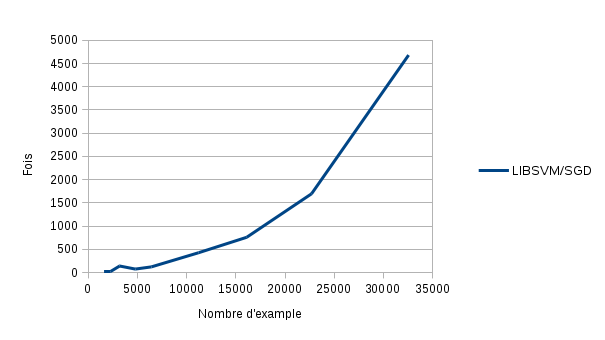
\includegraphics[width=100mm]{images/res}
\caption{Comparaison de la vitesse entre LIBSVM et SGD binaire}
\label{fig:res}
\end{figure}

\end{frame}


%=====================================================Slide 37
\begin{frame}{SVM et SGD multi-classes}

\begin{table}
\begin{center}
    \begin{tabular}{ | c | c | c | c | c | c |}
    \hline
    Données & SVM(\%) & SGD(\%) & SVM(s) & SGD(s) & $\frac{SVM(s)}{SGD(s)}$ \\ \hline
    
    mnist & 86.92 & 86.46 & 2810 & 0.72 & 3902.8 \\ \hline
    
    fr & 84.08 & 86.58 & 327 & 1.64 & 199.4 \\ \hline
    
    3d & 76.54 & 75.8 & 144 & 0.90 & 160 \\ \hline
    
    \end{tabular}
\end{center}
\caption{Comparaison entre LIBSVM et MC-SGD linaire et MC-SGD parallèle}
\label{tab:pmcsvm}
\end{table}

\end{frame}



%=====================================================Slide 38
\begin{frame}{Classification avec SVM et SGD multi-classes}

\begin{table}
\begin{center}
    \begin{tabular}{ | c | c | c | c | c | c |}
    \hline
    Données & SVM(\%) & SGD(\%) & SVM(s) & SGD(s) & $\frac{SVM(s)}{SGD(s)}$ \\ \hline
    
    S8c & 58.04 & 57.74 & 15 & 0.18 & 83.3 \\ \hline
    
    Cal 101 & 61.52 & 65.12 & 2873 & 106.95 & 26.9 \\ \hline    
    
    Cal 101 & 61.52 & 57.12 & 2873 & 74 & 38.8 \\ \hline   
    
    Cal 7 3D & 91.52 & 88.3 & 113.4 & 0.81 & 140 \\ \hline    
    
    \end{tabular}
\end{center}
\caption{Comparaison entre LIBSVM et MC-SGD parallèle pour la classification d'images}
\label{tab:pmcsvm-8scenes}
\end{table}

\end{frame}

\section{Conclusion}
%=====================================================Slide 40
\begin{frame}{Conclusion}
\begin{itemize}
\item Nous avons étudié le processus pour la classification d'images utilisant la méthode SVM, une méthode pour la classification générale
\item A partir de l'implémentation Pegasos, nous avons développé la méthode MC-SGD de classification multi-classes
\item MC-SGD est plus vite que SVM. Cette méthode correspond bien pour la classification d'image
\end{itemize}
\end{frame}

%=====================================================Slide 41
\begin{frame}{Conclusion (con)}
\begin{itemize}
\item Nous avons modifié l'implémentation Pegasos pour résoudre le problème de balance quand la base de données est de multi-classes
\item Pour économiser la ressource des ordinateurs multi-cœurs, nous avons paralléliser MC-SGD
\item Dans les testes que nous avons réalisé, le résultat de classification de SGD et SVM n'est pas beaucoup différent, tandis que SGD est beaucoup plus rapide que SVM
\item SGD s'adapte bien au problème de classification d'image
\end{itemize}
\end{frame}


%=====================================================Slide 42
\begin{frame}{Perspective}
\begin{itemize}
\item SGD est difficile de tester : choix des paramètres entrées
\item Le seuil de itération (nombre de cycle) de methode ($iter\ x\ nb\_ex\_per\_iter$) est de 500 à 50000, $\lambda$ est de 0.0001 à 0.5 SGD peut donner le bon résultat
\item Dans le future proche, nous étudierons pour chercher des paramètres optimales de la méthode
\item Nous testerons aussi des bases d'images plus grandes tel que ImageNet
\item Nous développerons pour SGD s'adapte à la classification de vidéos
\end{itemize}
\end{frame}



\end{otherlanguage}

% All of the following is optional and typically not needed. 
\section*{Références}
%=====================================================Slide 43
\begin{frame}{Références}
\begin{thebibliography}{9}

\bibitem{sss07} S.Shwartz, Y.Singer and N.Srebro \emph{ Pegasos: Primal esti-
mated sub-gradient solver for svm.}, Proceedings of the Twenty-Fourth International Conference Machine Learning, pp. 807-814. ACM (2007)

\bibitem{low99} David G. Lowe, \emph{Object Recognition from Local Scale-Invariant Features,} In proceeding of the 7th International conference of computer vision, pages 1150 - 1157, Corfou, Grèce, 1999.
 
\bibitem{vv95} V.Vapnik, \emph{The Nature of Statistical Learning Theory.}, Springer, New York (1995).

\bibitem{uk99} U.Krebel, \emph{Pairwise classification and support vector machines}, Support Vector Learning, Advances in Kernel Methods. pp.255–268. (1999).


\end{thebibliography}
\end{frame}

%=====================================================Slide 44
\begin{frame}
 \Huge Merci pour votre attention!!!!!
\end{frame}

\end{document}
